\section{Results}
\label{sec:results}

Statistical significance was achieved between our test case and our baseline regardless of whether we used random selection or parameter means. Between these two methods, taking the mean showed better accuracy, though not significantly so. Results varied between workflow runs but we observed differences in effect that increased the ending loss by as much as 5\% compared to the control and that decreased the ending loss as much as 20\%. 
There is little improvement after merging the networks following a short amount of time, however, there is significant improvement (including a quicker convergence) following a merge of two well-trained networks.
Though overall results were significant, we have observed bias in our testing towards partially trained models with similar parameter values. This aligns with our initial thoughts regarding the structure and shape of the parameter search space. Namely, for two local optima, it is not unlikely that another local optimum exists in a location between the two prior values.
\begin{figure}[h!]
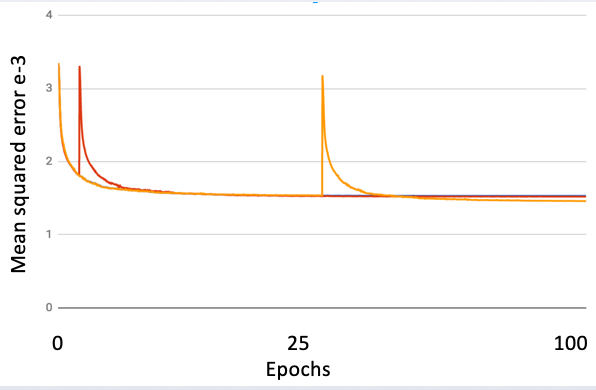
\includegraphics[width=\linewidth]{figures/loss.png}
\caption{Mean loss across 5 trial runs comparing the use of cross-over.}
\label{fig:results}
\end{figure}